\documentclass{beamer}

\usepackage{amsmath}
\usepackage{xspace}


% \newcommand\doubleplus{+\kern-1.3ex+\kern0.8ex}
\newcommand\doubleplus{\ensuremath{\mathbin{+\mkern-10mu+}}}


%% oracles
\newcommand{\ora}[1]{\ensuremath{\mathcal{O}\mathsf{#1}}\xspace}
%% algorithm
\newcommand{\algo}[1]{{\textsc{#1}}}
%%primitive algo
\newcommand{\primalgo}[1]{{\ensuremath{\mathsf{#1}}}\xspace}
%%primitive
\newcommand{\prim}[1]{{\ensuremath{\mathsf{#1}}}\xspace}
%%set
\newcommand{\setsym}[1]{{\ensuremath{\mathcal{#1}}}}
%%array
\newcommand{\arraysym}[1]{{\ensuremath{\mathsf{#1}}}}

\newcommand\N{\mathbb{N}}
\newcommand\F{\mathbb{F}}
% \newcommand\Gr{\mathbb{G}}


\def\mathperiod{.}
\def\mathcomma{.}



\newcommand*\set[1]{\{ #1 \}} % in text, we don't want {} to grow
\newcommand*\Set[1]{\left\{ #1 \right\}}
\newcommand*\setst[2]{\{ #1 | #2 \}}
\newcommand*\Setst[2]%
        {\left\{\,#1\vphantom{#2} \;\right|\left. #2 \vphantom{#1}\,\right\}}
% ``set such that''; puts in a vertical bar of the right height

\newcommand{\KeyGen}{\primalgo{KeyGen}}

% Why was this \prim before?
\newcommand{\VRF}{\primalgo{VRF}} 
\newcommand{\rVRF}{\primalgo{rVRF}} 

\newcommand{\Sign}{\primalgo{Sign}}
\newcommand{\Verify}{\primalgo{Verify}}
\newcommand{\Eval}{\primalgo{Eval}}
\newcommand{\Prove}{\primalgo{Prove}}
\newcommand{\Simulate}{\primalgo{Simulate}}
\newcommand{\Extract}{\primalgo{Extract}}


\newcommand{\In}{\primalgo{In}} 
\newcommand{\Out}{\primalgo{Out}} 
\newcommand{\PreOut}{\ensuremath{\primalgo{Out}_0}\xspace} 

\newcommand{\vk}{\ensuremath{\mathsf{vk}}\xspace}
\newcommand{\sk}{\ensuremath{\mathsf{sk}}\xspace}
\newcommand{\pk}{\ensuremath{\mathsf{pk}}\xspace}
\newcommand{\apk}{\ensuremath{\mathsf{apk}}\xspace}
\newcommand{\pkring}{\ensuremath{\setsym{PK}}}
\newcommand{\msg}{\ensuremath{\mathsf{msg}}\xspace}
\newcommand{\aux}{\ensuremath{\mathsf{aux}}\xspace}
\newcommand{\ctx}{\ensuremath{\mathsf{ctx}}\xspace}
\newcommand{\ringset}{\ensuremath{\mathsf{ring}}\xspace}



\newcommand\SNARK{\primalgo{SNARK}}
\newcommand\NIZK{\primalgo{NIZK}}


\newcommand{\adv}{\ensuremath{\mathcal{A}}\xspace}

\endinput

\newcommand{\evalprove}{\primalgo{EvalProve}}
\newcommand{\link}{{\primalgo{Link}}}
\newcommand{\update}{{\primalgo{Update}}}
\newcommand{\hashG}{\primalgo{H}_{\GG}}
\newcommand{\secreteval}{\primalgo{Secret}\eval}
\newcommand{\secretprove}{\primalgo{Secret}\prove}
\newcommand{\secretverify}{\primalgo{Secret}\verify}

\newcommand{\randsel}[0]{\ensuremath{\xleftarrow{\text{\$}}}}
\newcommand{\rel}{\ensuremath{\mathcal{R}}}


\endinput




\newcommand{\skvrf}{\ensuremath{\sk^{\mathsf{vrf}}}}
\newcommand{\pkvrf}{\ensuremath{\pk^{\mathsf{vrf}}}}
\newcommand{\skrvrf}{\ensuremath{\sk^{\mathsf{rvrf}}}}
\newcommand{\pkrvrf}{\ensuremath{\pk^{\mathsf{rvrf}}}}
\newcommand{\sksign}{\ensuremath{\sk^{\mathsf{sign}}}}
\newcommand{\pksign}{\ensuremath{\pk^{\mathsf{sign}}}}
\newcommand{\skksign}{\ensuremath{\sk^{\mathsf{kesign}}}}
\newcommand{\pkksign}{\ensuremath{\pk^{\mathsf{kesign}}}}
\newcommand{\pkssale}{\ensuremath{\pk^{\mathsf{ssale}}}}
\newcommand{\D}{\ensuremath{\Delta}}
\newcommand{\skzkvrf}{\ensuremath{\sk^{\mathsf{zkvrf}}}}
\newcommand{\pkzkvrf}{\ensuremath{\pk^{\mathsf{zkvrf}}}}


\def\comring{\ensuremath{\mathsf{comring}}\xspace}
\def\compk{\ensuremath{\mathsf{compk}}\xspace}


\title{Ethical identity, ring VRFs, and \\ zero-knowledge continuations}

\author{Jeffrey Burdges \and Handan Kilinc-Alper \and Alistair Stewart \and Sergey Vasilyev}
\date{15 Sept 2022}


\begin{document}


\maketitle


\begin{frame}

Zero-knowledge continuations..
	
\bigskip

Q: What is the fastest SNARK proof?

\bigskip

A: One that does not need (re)proving

\end{frame}



\begin{frame}

Ring VRF is a ring signature that's also a VRF.

\bigskip 

A [ring] verifiable random function (VRF) is a [ring] signature that proves evaluation of a pseudo-random function (PRF) determined by the actual key pair.


\end{frame}



\begin{frame}{EC VRF}

$\mathsf{ECVRF}.\Verify(\msg,\aux,\pk,(\Out,R,R_\msg,s))$

$$ \begin{aligned}
\In &= H_{\mathcal{G}}(\msg) \\
c &= H(\msg,\aux,\pk,R,R_\msg) \\
s \, \In &= R' + c \, \Out \\
s \, G &= R + c \, \pk \\
\end{aligned} $$

\end{frame}



\begin{frame}{Pederson VRF}
	
$\mathsf{PedersonVRF}.\Verify(\msg,\aux,\compk,(\Out,R,R_\msg,s,t))$
	
$$ \begin{aligned}
\In &= H_{\mathcal{G}}(\msg) \\
c &= H(\msg,\aux,\pk,R,R_\msg) \\
s \, \In &= R' + c \, \Out \\
t \, K + s \, G &= R + c \, \compk \\
\end{aligned} $$
	
\end{frame}



\begin{frame}
	
$\mathsf{Groth16}.\Verify(X,(A,B,C))$
	
$$ e(A,B) = e([\alpha]_1, [\beta]_2) \cdot e(X, [\gamma]_2) \cdot e(C, [\delta]_2) $$

\pause\medskip

Add $K_\delta := {\gamma\over\delta} K$ to trusted setup

$$ \begin{aligned}
X' &:= X + b K \\
A' &:= {1 \over r_1} A \\
B' &:= r_1 B + r_1 r_2 [\delta]_2 \\
C' &:= C + r_2 A + b K_\delta \\
\end{aligned} $$

\end{frame}



\begin{frame}

$$ \mathsf{Groth16} \Setst{ \sk_0 + \sk_1 2^{128}, \comring }{
    \exists d,o \textrm{\ s.t.\ }
	\genfrac{}{}{0pt}{}{ \sk_0 J_0 + \sk_1 J_1 + d J_2 }{ \in_o \comring }
} $$

\pause\bigskip 

$$ \mathsf{Groth16} \Setst{ \sk_0 + \sk_1 2^{128}, J_\pk }{ 
	\exists d \textrm{\ s.t.\ }
	J_\pk = \sk_0 J_0 + \sk_1 J_1 + d J_2
} $$

\end{frame}



\begin{frame}{Identity}

User agent: \\ \medskip

1st) validates TLS cert of ``site.com'', including CT logs. \\ \medskip

2nd) sends ring VRF signature with $\msg = \mathtt{``site.com``}$. \\ \medskip

\pause\bigskip\bigskip 

What happens if we use $\msg = \mathtt{``site.com``} \doubleplus \mathsf{month}$?

\end{frame}



\begin{frame}

``No civilization can possibly survive to an interstellar spacefaring \\ \smallskip
\hspace{1pt} phase unless it limits its numbers'' (and its consumption) \\ \medskip
--- Carl Sagan

\pause\bigskip\bigskip 

Anonymous rationing uses $\msg = \mathtt{``site.com``} \doubleplus \mathsf{week} \doubleplus \mathsf{counter}$ \\
\hspace{1pt} And treats outputs as short lived nullifiers.

\pause\bigskip\bigskip 

Important: Ring membership can be transparent!  No fraudulent certificates!

\end{frame}



\begin{frame}{Sassafras}

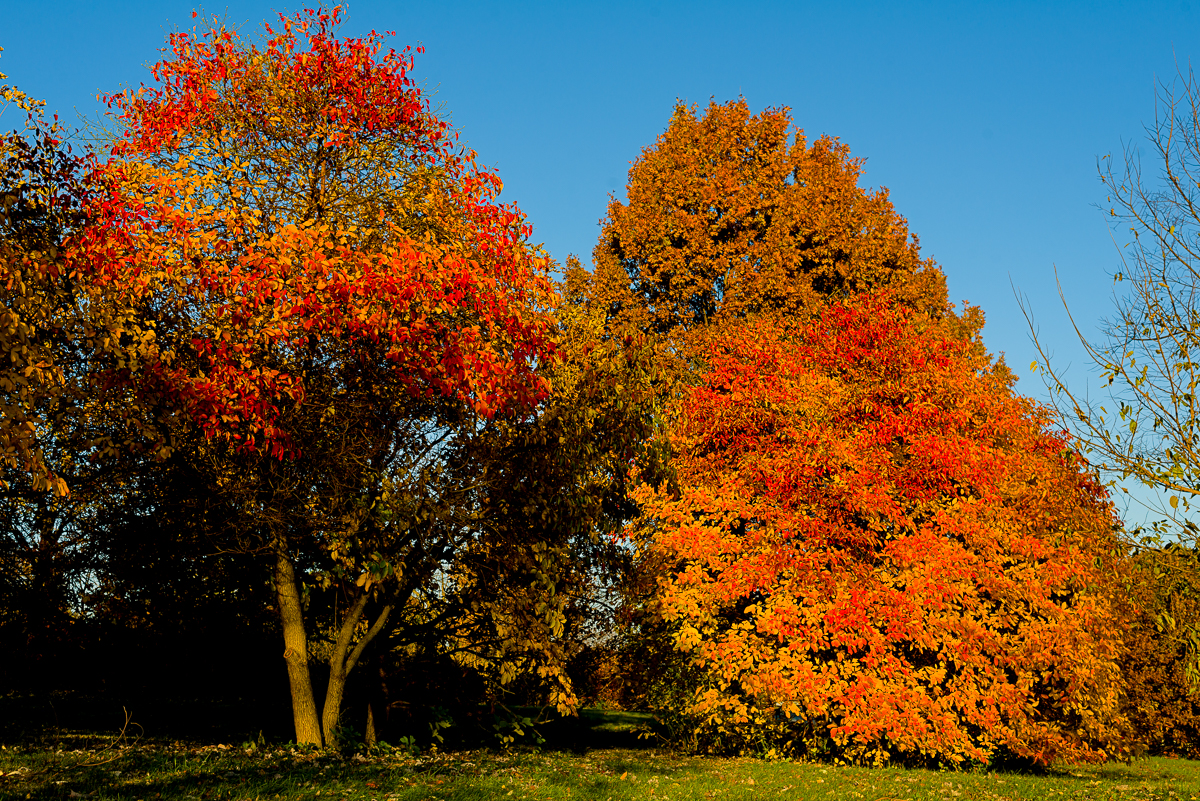
\includegraphics[width=\textwidth]{Sassafras-albidum.jpg}

\end{frame}



\begin{frame}

SSLE = Secret single leader election

\bigskip\bigskip

Sassafras: Semi-anonymous sortition of staked assignees for fixed-time rhythmic assignment of slots

\pause\bigskip\bigskip

It's basically block production by cards against humanity.

\end{frame}



\begin{frame}
\end{frame}



\end{document}








\begin{frame}


		
\end{frame}




